\section{Introduction}
\label{sec:introduction}

%Reconstruction of neuronal morphology is important for brain studies. 
A blue print of the brain architecture, including the morphology and interconnectivity of neuronal populations, allows for measuring and visualizing neuronal structure, understanding neuronal identity, and determining potential connectivity.
Therefore, complete reconstruction of neuronal populations from ultra-scale brain images is essential to investigate the mechanism of the nervous system, analyze brain changes, and facilitate our understanding of brain diseases such as dementia and Alzheimer's disease~\cite{Petrella2003, Giorgio2013}.
One of the key techniques in this endeavor is optical microscopy (OM), which allows detailed visualization of neurons and makes the reconstruction of every neuron possible~\cite{Senft2011}, as shown in Fig.~\ref{fig:brain}.
However, despite numerous efforts devoted, this task is still one of the main challenges in computational neuroscience.

\begin{figure}[t]
	\centering
	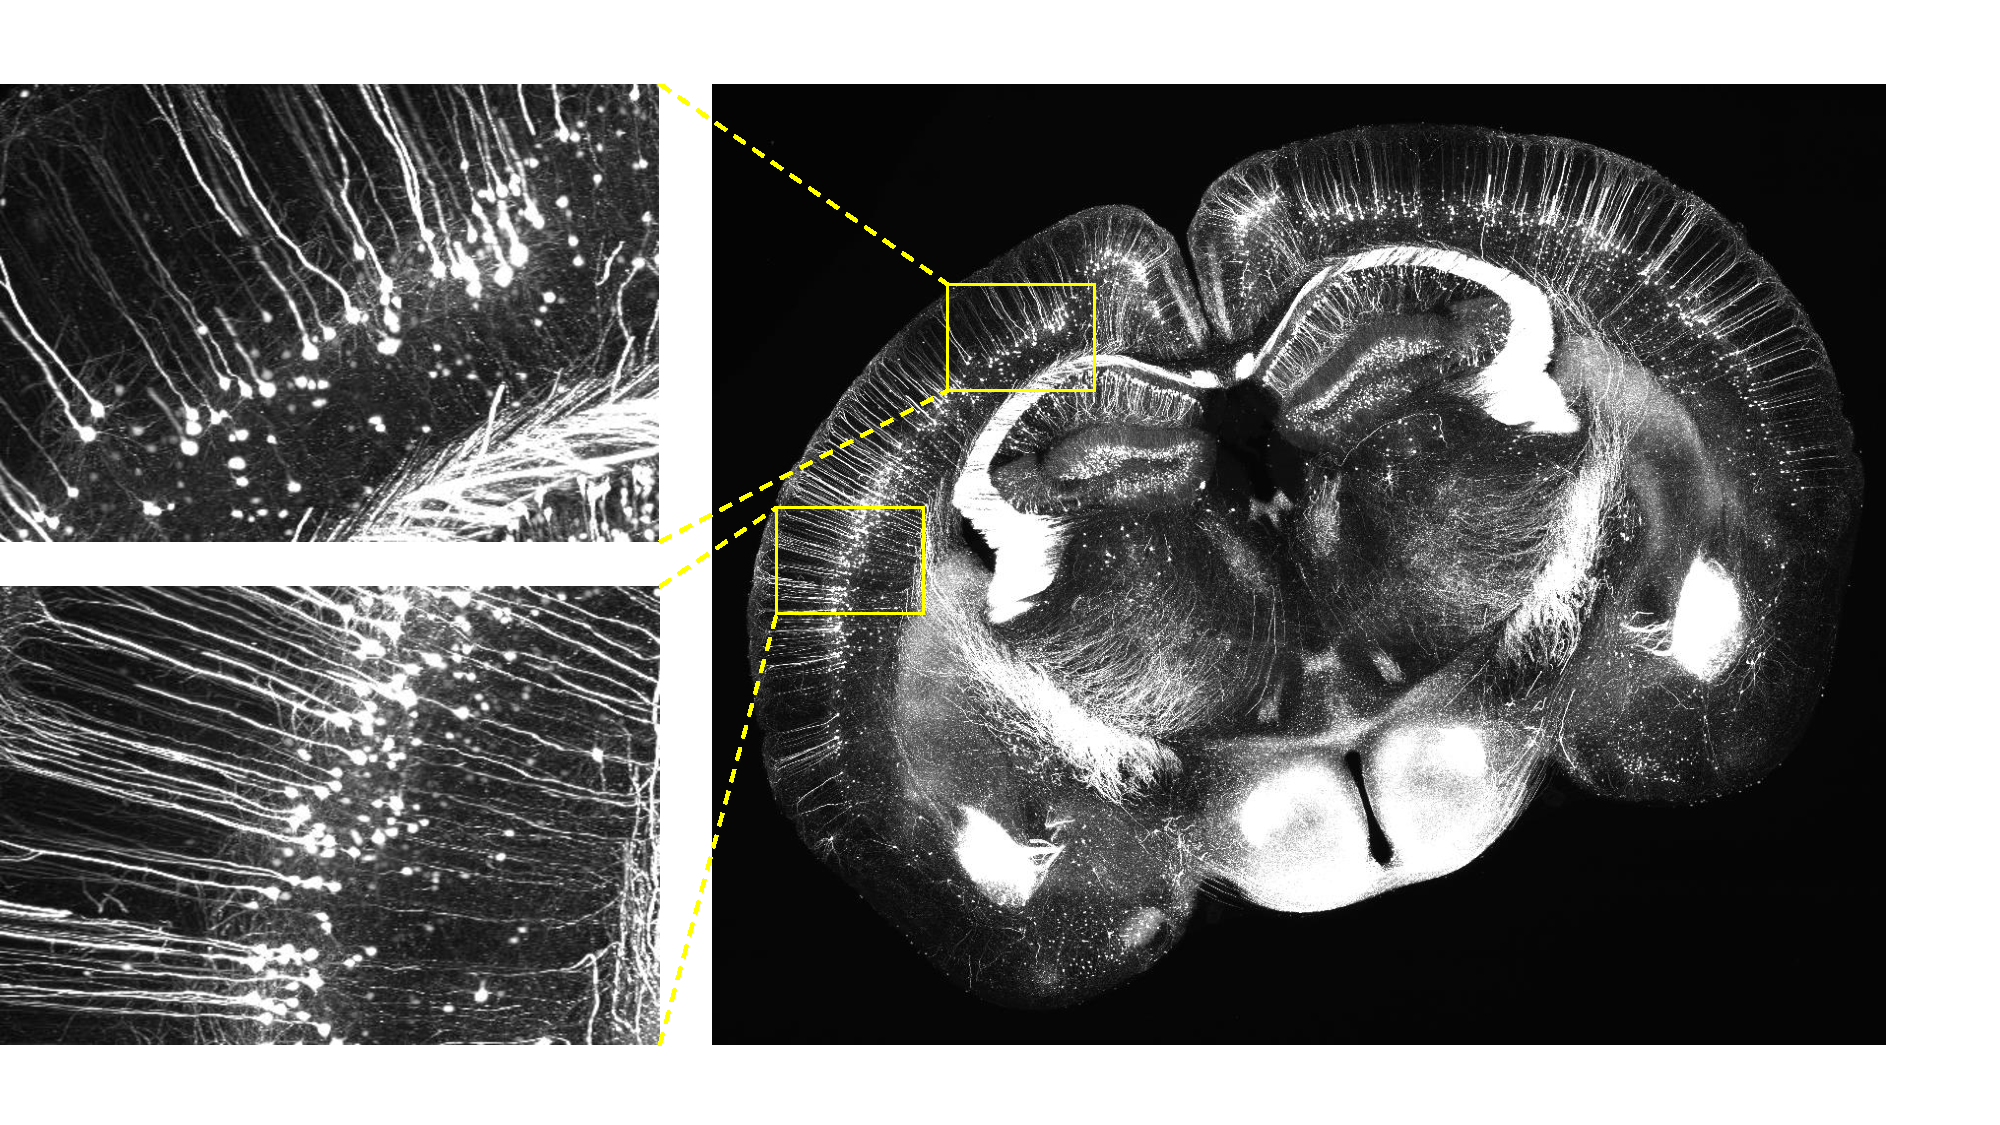
\includegraphics[width=1\columnwidth]{./Illustrations/brain2.pdf}
	\caption{A 3D OM image for a mouse brain slice captured by the VISoR imaging system~\cite{Wang2019}. The large density of neurons, low contrast, image noises, and huge volume pose significant challenges for automatic reconstruction of neuronal populations from the ultra-scale image.}	
	\label{fig:brain}
\end{figure}

The challenges in ultra-scale neuronal population reconstruction are mainly caused by complex morphology of neurons, low quality, and huge volume of OM brain images.
Due to the complicated process of imaging acquisition and the uneven distribution of fluorescence markers in neurons, the voxel intensities vary dramatically in highly noisy and inhomogeneous environments.
Moreover, to detail the structure of neurons in the brain, OM images in high resolution are required. Such an image typically contains trillions of voxels. It is even impractical to directly load the entire image into a computer memory before reconstructing neurons.
In the other hand, manual reconstruction of neuronal populations from ultra-scale brain images is an extremely laborious and time-consuming task as well.
Moreover, sophisticated knowledge of neuron morphology is also required for manual reconstruction.
%
Therefore, an effective and automatic reconstruction algorithm for ultra-scale neuronal population in these challenging situations is greatly desired in practice.
 % 
 
 
Attempts have been made for neuron reconstruction from large-scale OM images in recent years, such as Neuron Crawler~\cite{Zhou2015}, UltraTracer~\cite{Peng2017} and MEIT~\cite{Wang2018}.
A common solution is to divide the large-scale image into blocks and then trace neurons block by block.
Despite their great improvements in this task, several limitations still remain.
%
One main bottleneck is that the base tracers used for neuron tracing in image blocks typically employ a series of traditional image processing algorithms such as binarization, fast marching, ray-shooting, etc. 
Unfortunately, these algorithms using hand-crafted features and rules have difficulty in reconstructing neurons from low-contrast and noisy image blocks.
To improve the reconstruction quality, deep learning techniques have been adopted in neuron reconstruction recently~\cite{Xu2016, Li2017, Zhou2018, Kozinski-MIA2020}. 
However, these approaches require huge amount of manually annotated data to train the deep neuron segmentation networks.
%

Compared with manual annotations, the reconstruction results by conventional algorithms effectively provide approximate locations of neurons. 
Although these voxels may not cover all neurons precisely, they provide important cues for obtaining complicated patterns of neurons.
Therefore, we propose a progressive learning scheme for neuronal population reconstruction (PLNPR) to take advantage of both conventional methods and deep learning techniques.
More specifically, we employ conventional methods to produce pseudo-labels for training a deep neural network for neuron segmentation. 
The network is expected to learn more comprehensive features of neurons from noisy labels. 
With a more powerful DNN for segmenting neurons, the neuron reconstruction using conventional tracers could be improved. 
Then we progressively refine the segmentation DNN with better neuron reconstruction results as pseudo labels and reconstruct more complete neurons with better neuron segmentation.
We first investigate this concept in our preliminary work \cite{Zhao2019} on a few image blocks. 
In this work, we apply PLNPR on dense neuron population reconstruction from an ultra-scale OM image. 

Another limitation of existing large-scale neuron reconstruction methods~\cite{Zhou2015, Peng2017, Wang2018} is that they mainly focus on single neuron reconstruction. 
%
For dense neuronal population reconstruction from ultra-scale images, dense neurites may cross with each other, making the neuron tracing much more challenging in low-contrast and noisy OM images. 
% 
Following the commonly used block-by-block framework, we introduce UltraNPR, which utilizes our PLNPR approach as the base tracer in blocks, and design novel tracing and fusion strategies for reconstructing dense neuronal populations.
%
We start local reconstruction using our PLNPR in the blocks where soma can be detected, and propagate a group of neurite tips as pseudo somas for neighboring blocks to trace the neuron population. 
%
There are over-tracing and topological discrepancy in the reconstructed neurites in adjacent blocks. 
We design a fusion method with spatially varying confidences in order eliminate the tracing errors that usually occur at boundary regions of local blocks.   


In summary, we propose PLNPR, a progressive learning framework that integrates traditional tracing methods and deep segmentation networks for neuron population reconstruction without using manual annotations.
%
Then we introduce UltraNPR by integrating PLNPR with adaptive block-wise propagation and fusion strategies which can reconstruct dense neuronal populations from trillions of voxels in ultra-scale OM images. 
%
In order to evaluate our method, we build a dataset ``VISoR-40" which consists of 40 OM image blocks from mouse cortical regions. Manual annotations of eight blocks in the dataset are available for the community. Extensive experiments on our VISoR-40 dataset and the BigNeuron dataset demonstrate the effectiveness and superiority of our progressive learning algorithm for both neuronal population reconstruction and single neuron reconstruction.
The reconstructed neuron population from an ultra-scale image of a mouse brain slice shows the robustness of our UltraNPR.




%In this work, we introduce UltraNPR, an algorithm designed for reconstructing dense neuronal populations from large-scale or even ultra-large-scale images. UltraNPR reconstructs neuronal populations by progressively improving the completeness of neuronal structure block by block.
%
\delete{Firstly, the large-scale raw image is divided into blocks of the same size.
Since somas are where signals from the dendrites are joined and pass on, UltraNPR begins the reconstruction from the blocks that contain somas.
% which can be detected using existing soma detection methods.
For robust reconstruction from low-quality images, our PLNPR method is applied to trace neurons in each block.
Based on the reconstruction results in already-reconstructed blocks, UltraNPR automatically and adaptively searches the next block to trace.
%For each block containing somas, this reconstruction procedure repeats until no new terminal tips could be detected or the next block contains somas.
%Finally, UltraNPR analyzes the reconstruction results in all blocks, and assembles the matched neurites from adjacent blocks to obtain the final complete neuronal population reconstruction. In our implementation, 
Finally, a fusion algorithm is designed to make the fragmented neurites of a neuron from adjacent blocks can be assembled continuously and smoothly.
In this way, UltraNPR is capable of exploring a large-scale image for neuronal population reconstruction.



%%%%%%%%%%%%%%%%%%%%%%%%%%%%%%%%%%%%%%%
In summary, we make the following contributions in this work. 
\begin{enumerate}
\item We propose a general progressive learning framework that can integrate existing neuron tracing and deep segmentation networks for neuron reconstruction without using manual annotations.

\item We integrate our PLNPR with a block-wise propagation and fusion strategy which can reconstruct dense neuronal populations from trillions of voxels in an image slice. 

\item We build a dataset ``VISoR-40" which consists of 40 OM image blocks from mouse cortical regions. Manual annotations of eight blocks in the dataset are available. 
%which consists of 40 OM images from mouse cortical regions and contains about 400 neuronal trees. Publishing this dataset will strongly support the study of deep neural networks for microscopic explorations.
\item Extensive experiments on our VISoR-40 dataset and the public BigNeuron dataset demonstrate the effectiveness and superiority of our progressive learning algorithm for both neuronal population reconstruction and single neuron reconstruction.
\end{enumerate}
}
 